\chapter{Architecture}

\hspace{-.6cm}Voici le diagramme de classe général, celui-ci ne représente que le cadre de l'API :
\begin{figure}[H]
\begin{center}
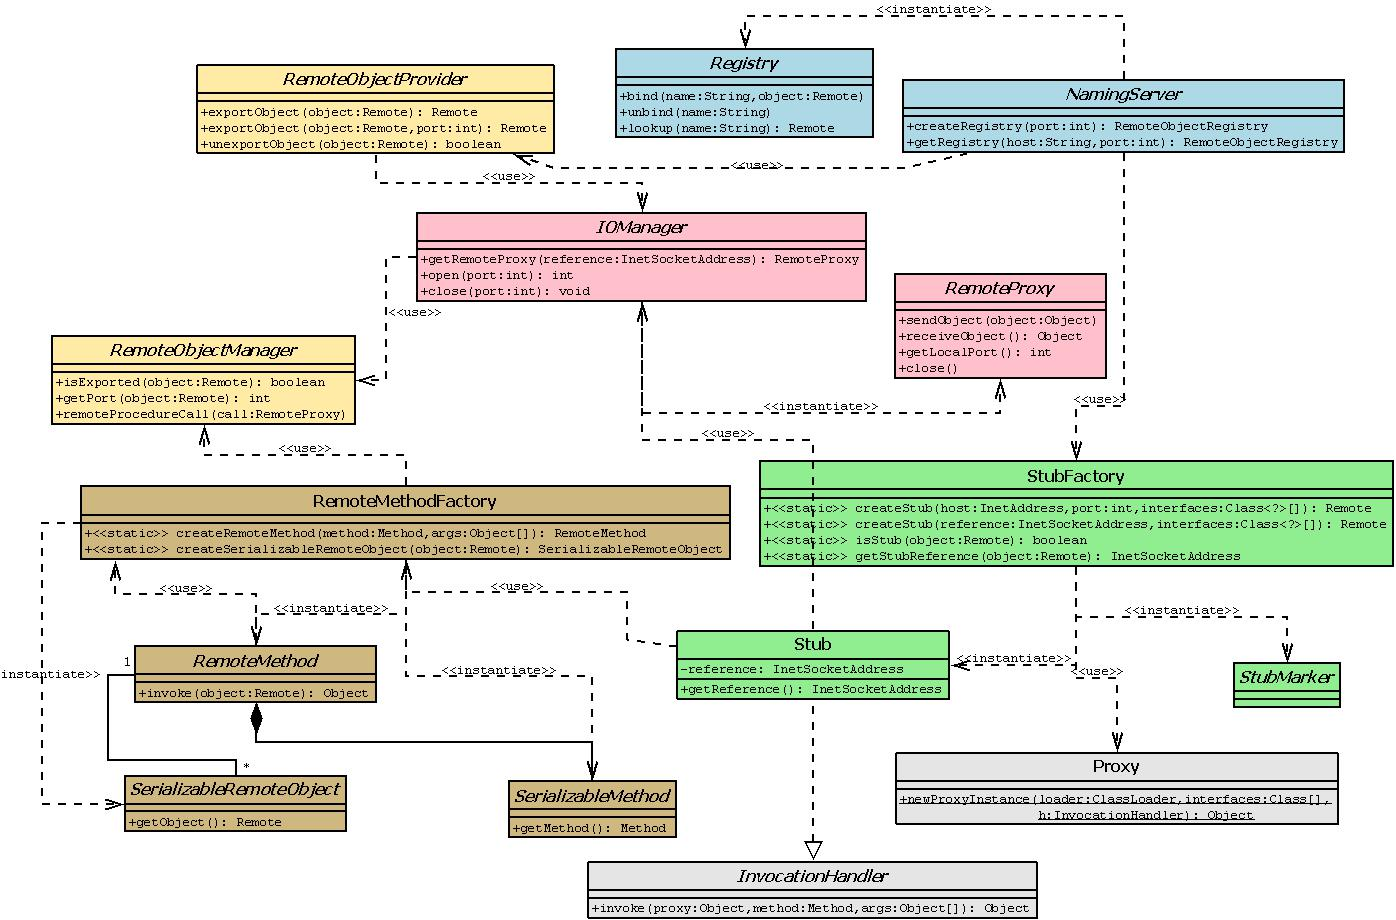
\includegraphics[scale=0.42,angle=90]{img/diag_classes.jpeg}
\caption{Diagramme UML de classes}
\end{center}
\end{figure}
\medskip
\hspace{-.6cm}On peut distinguer clairement 5 parties différentes :
\begin{itemize}
\item Serveur de nom
\item Partage d'objets
\item Couche réseau
\item Appels distants
\item Stub
\end{itemize}
\medskip

On identifie un objet partagé sur le réseau grâce à son adresse IP et le port (InetSocketAddress) sur lequel il reçoit les appels distants.

\section{Serveur de nom}
\hspace{-.6cm}Le fournisseur de registre exporte en même temps que de créer un registre distant. De même, il créé un stub quand on lui en demande un.

\section{Partage d'objets}
L'interface RemoteObjectManager est interne à l'API, elle n'est pas destinée à être utilisée par l'utilisateur lambda. Elle permet à l'usine d'appels distants de vérifier si les objets manipulés en paramètre ou en retour sont bien exportés, et si c'est le cas, d'obtenir leur port d'écoute. Elle permet aussi à la couche de communication de faire remonter un appel distant vers l'objet partagé.

\section{Couche réseau}
L'interface RemoteProxy est destinée à encapsuler un socket, fournit par un IOManager qui se charge d'ouvrir, d'écouter et de fermer des ports.

\section{Stub}
\hspace{-.6cm}Grâce à l'API de réflexion java.reflect, il est possible de créer des stubs dynamiquement.

\section{Appels distants}
A noter qu'une instance de RemoteMethod doit être sérialisable et contenir tout les paramètres nécessaires à l'éxécution de la méthode distante (ou appel distant) sur l'objet partagé spécifié en paramètre.

